\chapter{Overlapping, heterogeneous age groups: atrial fibrillation}
\label{applications-age_groups}
\chapterprecis{Mohammad H. Forouzanfar, Abraham D. Flaxman, Hannah M. Peterson, Mohsen Nagavi, and Sumeet Chugh}

Like many conditions analyzed in the GBD 2010 Study, atrial
fibrillation (AF) has no standard set of age groups for reporting.  The
meta-analysis of the data collected in systematic review must address
these heterogeneous age groups in some way. AF provides a prototypical
example of this, one where the results of the choice to
use an age-standardizing model can be compared with those of other possible
choices.  This chapter compares the estimates produced for AF
prevalence and incidence using an age-standardizing model with those
from a midpoint model.

AF is the most common type of cardiac arrhythmia.  Chaotic and
irregular heart rhythms originating in the atria cause poor blood flow
to the body.  The duration of AF episodes varies greatly.
Paroxysmal AF is occasional, with attacks lasting a few minutes or hours,
whereas persistent AF and permanent AF are chronic, continuing for
days with or without self-termination.  Symptoms include
heart palpitations, lack of energy, dizziness, shortness of breath, and
chest discomfort, although some cases of AF are
symptomless.  AF may occur at any age, with increasing risk for older
ages, and is uncommon in children.  Other heart diseases tend to be
the underlying cause of AF.  AF is associated with coronary heart
disease, hypertensive heart disease, valvular heart disease, heart
failure, cardiomyopathy, obesity, and metabolic disorders such as
diabetes and hyperthyroidism. \cite{rich_epidemiology_2009,
  rho_asymptomatic_2005, fuster_acc/aha/esc_2006, radford_atrial_1977}
%  TK_ref_from_Mehrdad}

The GBD 2010 Study defines AF as a patient having at least one episode
confirmed by a physician.  The systematic review of AF collected $3942$
data points, of which $247$ were from countries in Western Europe.  We
will consider only the Western European data in this chapter.
We have $20$ data points on disease incidence and $147$ on prevalence.
As seen from figure~\ref{fig:app-af data}, AF has
heterogeneous and overlapping age groups.  Without access to the
microdata needed to re-create homogeneous age groups, combining all
these data must rely on age-group modeling, as described in
chapter~\ref{chap:age_group_model}.

    \begin{figure}[h]
        \begin{center}
            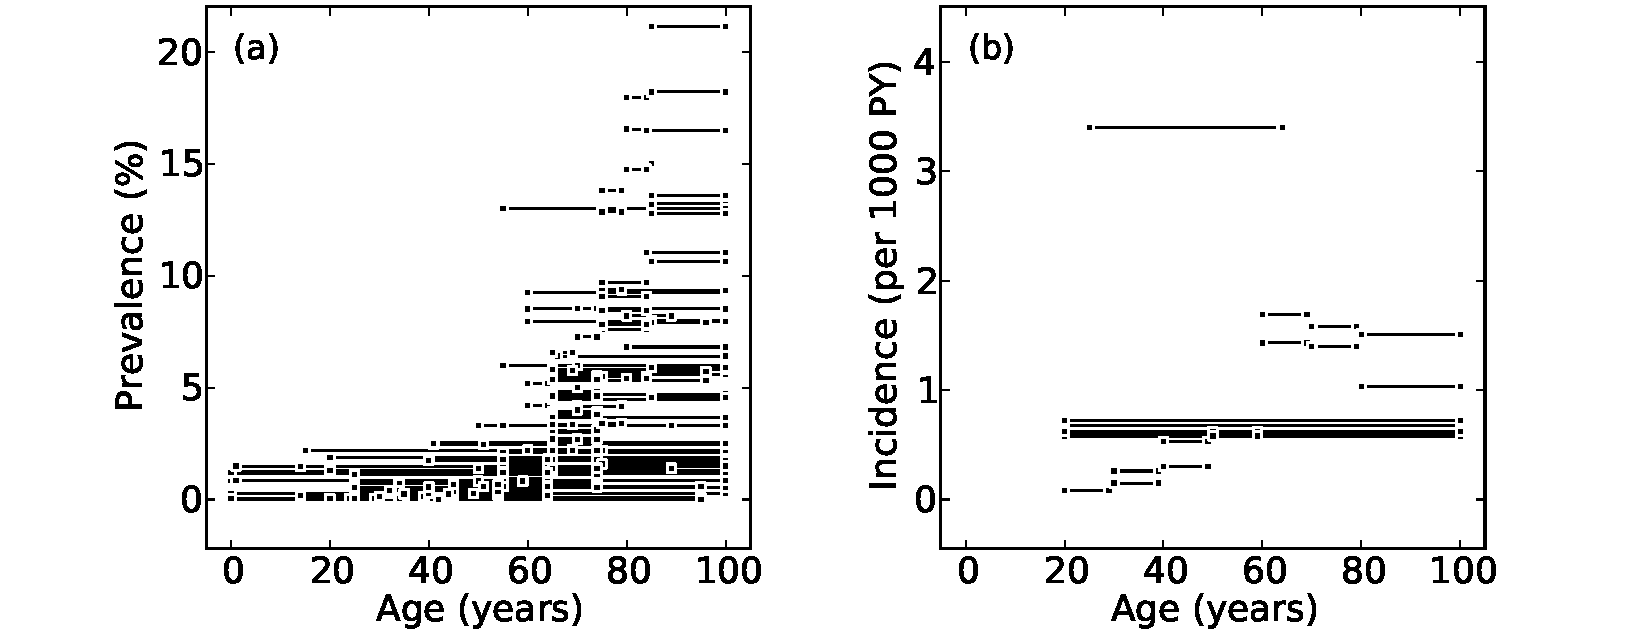
\includegraphics[width=\textwidth]{af-data.pdf}
            \caption[Systematic review data of atrial fibrillation.]{Data for
              prevalence and incidence of AF in
              Western European males.  This is a typical example of
              the sort of heterogeneous and overlapping age groups
              collected in systematic review.}
            \label{fig:app-af data}
        \end{center}
    \end{figure}

As discussed in section~\ref{theory-age_group_model-mp_model},
the simplest approach to modeling heterogeneous age groups is to apply
each age-specific rate measurement to the midpoint of the age interval.
Another solution to the heterogeneous age groups is to use age standardizing
(section~\ref{age-standardizing}).  Age standardizing adds age weights to the age-specific rate according
to population structure.  The age-standardizing model uses a common
age pattern for all studies so that the age weights are the same for
all country-years, as discussed in more detail in section~\ref{age-standardizing}.

As the prevalence estimates in figure~\ref{fig:app-af srt p} show,
model choice changes the estimates.  In estimates before age 80,
differences are minimal, but in estimates for older ages, where the
data are sparser and noisier, the differences are substantial.

    \begin{figure}[h]
        \begin{center}
            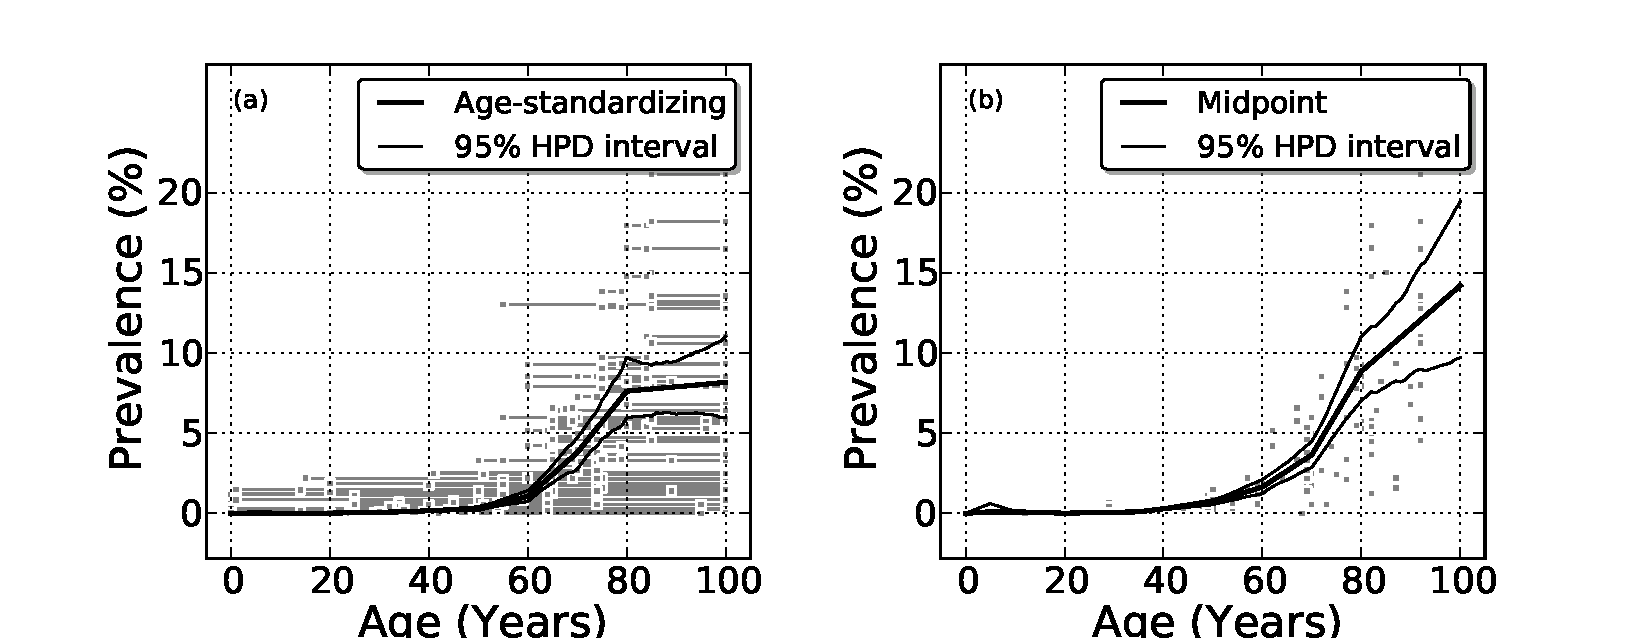
\includegraphics[width=\textwidth]{af-mp_v_hetero_srt_p.pdf}
            \caption[Comparison of prevalence estimates for atrial fibrillation
              using an age-standardizing model and midpoint model.]{Comparison
              of estimates of prevalence of AF for Western European
              males in 1990: (a) data and estimates for the
              age-standardizing model; (b) data and estimates for the
              midpoint model.}
            \label{fig:app-af srt p}
        \end{center}
    \end{figure}

Without additional information, one cannot say which model is preferred.
Further investigation with incidence does not provide much insight.
Figure~\ref{fig:app-af srt i} shows that, like the prevalence estimates, the
incidence estimates are similar in younger ages but are markedly different
in older ages.  The age-standardizing model also produces estimates with a
smoother age pattern.

    \begin{figure}[h]
        \begin{center}
            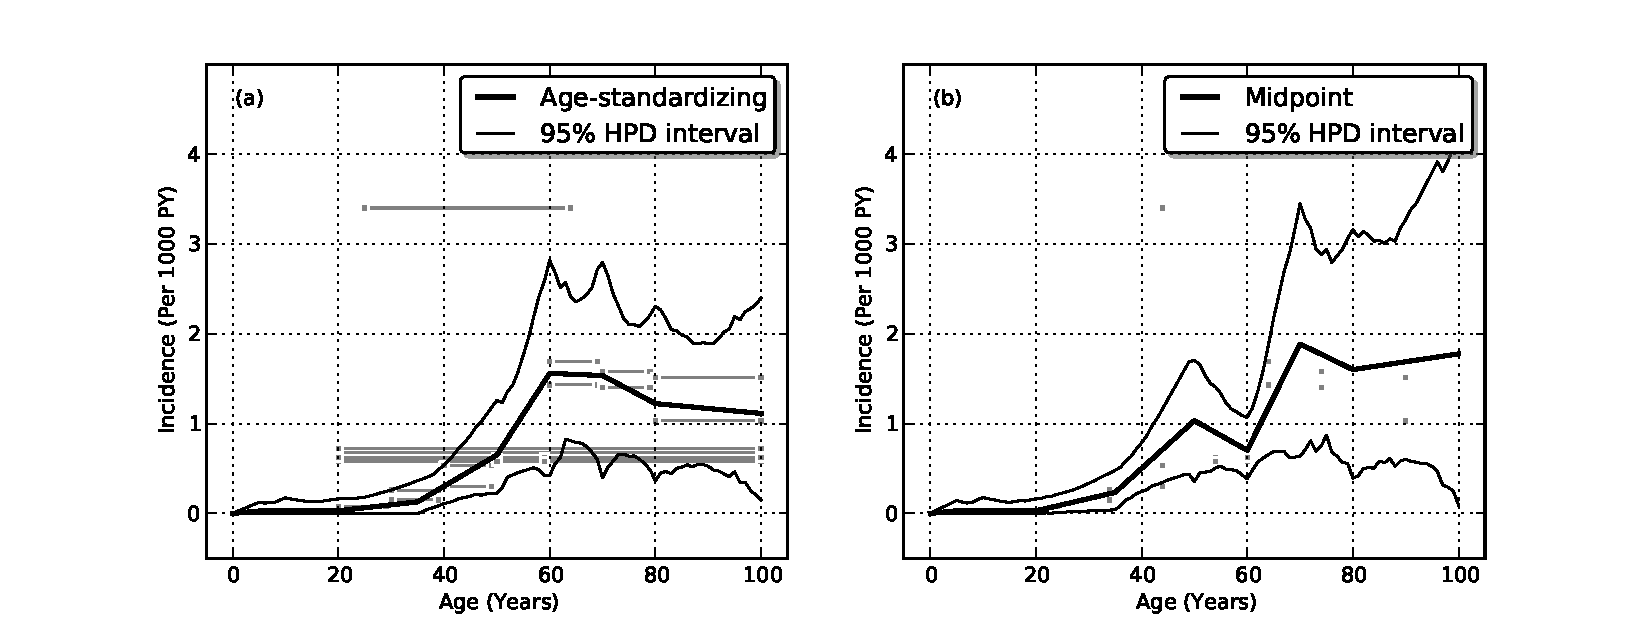
\includegraphics[width=\textwidth]{af-mp_v_hetero_srt_i.pdf}
            \caption[Comparison of incidence estimates for atrial fibrillation
              using an age-standardizing model and midpoint model.]{Comparison of estimates of incidence of AF for
              Western European males in 1990: (a) data and
              estimates for the age-standardizing model; (b) data and
              estimates for the midpoint model.}
            \label{fig:app-af srt i}
        \end{center}
    \end{figure}

Using all available data in a compartmental model, including the
limited available data on excess mortality, with-condition mortality,
and cause-specific mortality, is a way to combine the data on
incidence and prevalence to produce internally consistent estimates by
modeling all parameters simultaneously.  The prevalence estimates
from this model are preferred to those from a spline model of prevalence alone
because the compartmental model incorporates additional data.  Compartmental models are
discussed in more detail in
section~\ref{sys-dynamics}.  Figure~\ref{fig:app-af age-stand} shows
consistent prevalence and incidence estimates from the
age-standardizing compartmental model.

The compartmental model estimates for incidence in
figure~\ref{fig:app-af age-stand} are very different from the spline
model estimates.  Unlike the spline models, the compartmental model
estimates for incidence do not go through all the data.  This is
because the compartmental model requires internal consistency;
that is, for every prevalence case there must be a matching incidence event.
The compartmental model shows that these levels of prevalence cannot
be achieved with the levels of incidence the data show.

    \begin{figure}[h]
        \begin{center}
            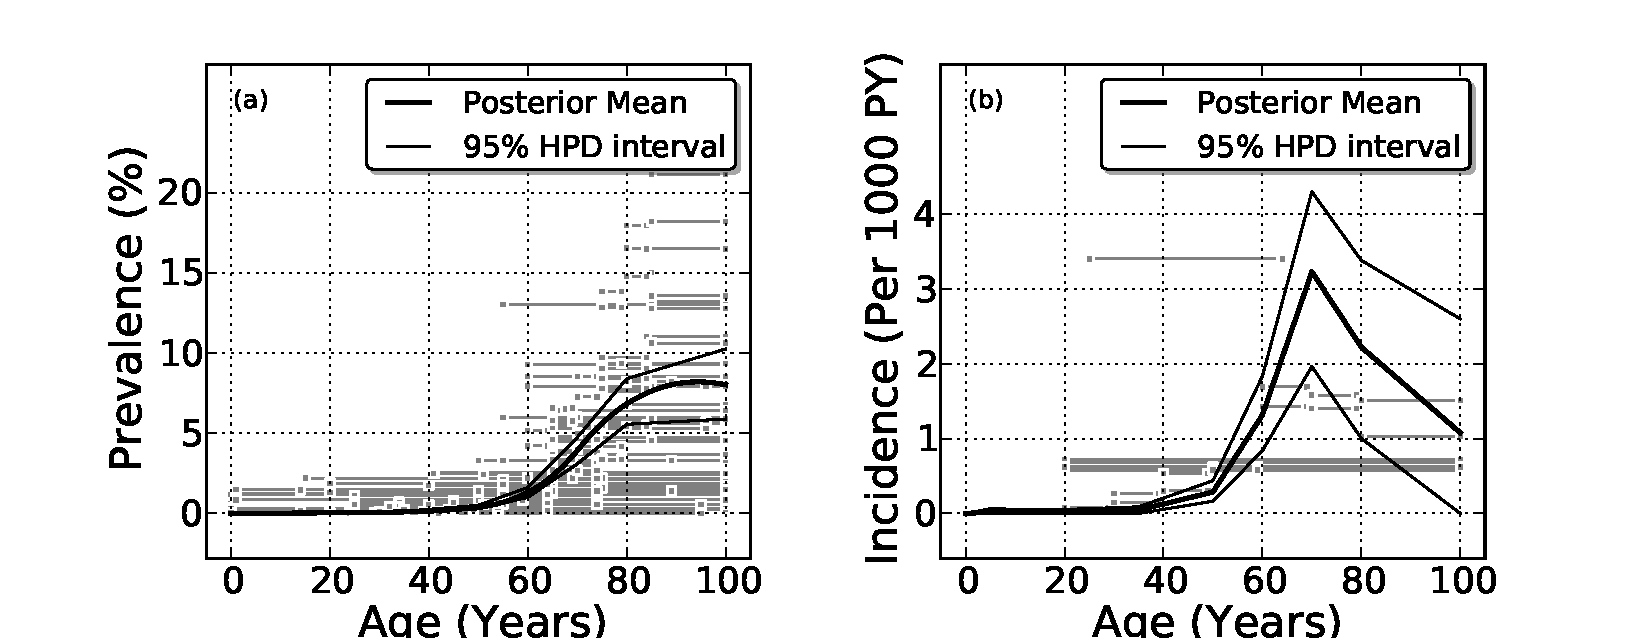
\includegraphics[width=\textwidth]{af-best_model.pdf}
            \caption[Estimates of atrial fibrillation
              using an age-standardizing compartmental
              model.]{Estimates of AF in Western European males in 1990
              using an age-standardizing compartmental model for (a)
              prevalence and (b) incidence.}
            \label{fig:app-af age-stand}
        \end{center}
    \end{figure}

Figure~\ref{fig:app-af compare} compares the prevalence and incidence
estimates from the age-standardizing compartmental model with those from the
midpoint compartmental model.  As with the spline models, the
estimates differ substantially only in the oldest ages.

    \begin{figure}[h]
        \begin{center}
            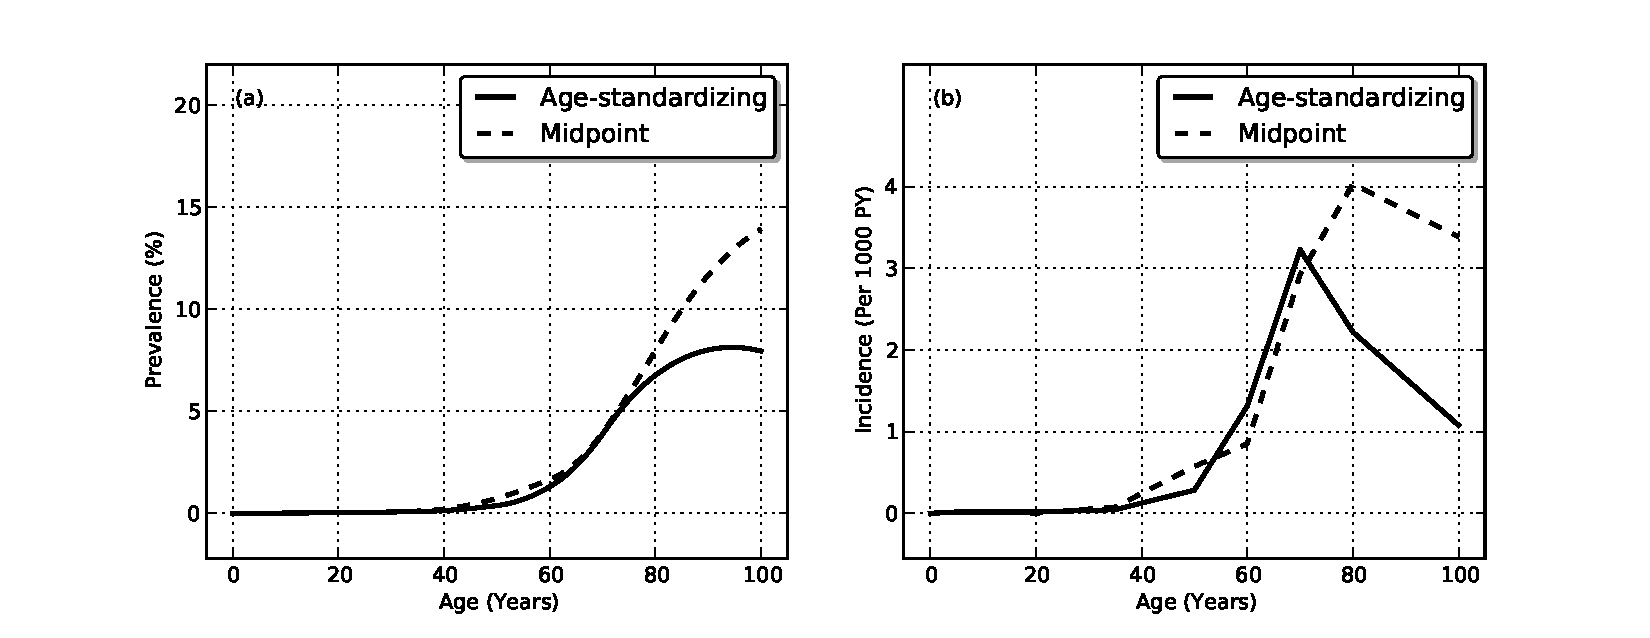
\includegraphics[width=\textwidth]{af-mp_v_hetero.pdf}
            \caption[Comparison of prevalence and incidence estimates for
              atrial fibrillation using an age-standardizing model and midpoint model.]{Comparison of the estimated (a) prevalence and (b) incidence
              in Western European males with AF in 1990
              using age standardizing and midpoint compartmental models.}
            \label{fig:app-af compare}
        \end{center}
    \end{figure}

The choice of age-group model has implications for disease estimates.
Estimated age pattern, trends, and levels can differ between the
midpoint and age-standardizing models.  The age-standardizing model is a
unique feature of the approach developed in this book,
and allows more appropriate use of systematic review data than simply
applying the measurement to the midpoint of the age interval.
